
\documentclass[twoside,onecolumn]{article}

\usepackage{blindtext} % Package to generate dummy text throughout this template 

%\usepackage[sc]{mathpazo} % Use the Palatino font
\usepackage[T1]{fontenc} % Use 8-bit encoding that has 256 glyphs
\linespread{1.05} % Line spacing - Palatino needs more space between lines
\usepackage{microtype} % Slightly tweak font spacing for aesthetics
\usepackage{float}
 \usepackage{amsmath}
 \usepackage{booktabs}
 \usepackage{amssymb}
 \usepackage{amsthm}
 \usepackage{tabularx} %tabelle
 \usepackage{tikz} %circuiti
 \usepackage{enumerate}
 \usepackage{pgfplots}
 \usepackage{subcaption}
\usepackage[toc,page]{appendix}
 \usepackage[export]{adjustbox}
 \usepackage{caption}
 \usepackage{subfig}
 \usepackage{sidecap}
 \usepackage{algorithm}

 \usepackage{graphicx}
 \theoremstyle{definition}
  \usepackage{multicol}
  \usetikzlibrary{arrows}
  \usepackage{algpseudocode}

  
\usepackage[english]{babel} % Language hyphenation and typographical rules

\usepackage[hmarginratio=1:1,top=32mm,columnsep=20pt]{geometry} % Document margins
\usepackage[hang, small,labelfont=bf,up,textfont=it,up]{caption} % Custom captions under/above floats in tables or figures
\usepackage{booktabs} % Horizontal rules in tables

\usepackage{lettrine} % The lettrine is the first enlarged letter at the beginning of the text

\usepackage{enumitem} % Customized lists
\setlist[itemize]{noitemsep} % Make itemize lists more compact

\usepackage{titlesec} % Allows customization of titles
\titleformat{\section}[block]{\large\scshape\centering}{\thesection.}{1em}{} % Change the look of the section titles
\titleformat{\subsection}[block]{\large}{\thesubsection.}{1em}{} % Change the look of the section titles

\usepackage{hyperref} % For hyperlinks in the PDF

\title{Homework 2: Pseudo Random Number Generators } % Article title
\author{Nicole Zattarin}
\date{} 
\begin{document}

% Print the title
\maketitle

\begin{abstract}
Random Number Generators (RNG) are a fundamental, yet quite delicate aspect of simulation. RNGs are necessary in most of scientific simulations to generate random variables which correspond to the real event that we aim to simulate. Nevertheless, it is impossible to generate sequences of real random numbers without exploiting an external source of randomness, e.g. Quantum RNGs, because the behaviour of our algorithms is essentially deterministic. Therefore, we refer to random numbers generators based on an algorithmic approach as Pseudo RNGs. In this report we explore both all the limitations connected to the generation of pseudo random numbers and different methods to design PRNGs.

\end{abstract}



\section{Linear congruence}
Let us consider a first example of PRNG: given a seed $s$ and two parameters $a$ and $m$, computes a sequence of pseudo random number as follows:
\begin{equation}
x_n = \frac{sa^n\mod m}{m},
\end{equation}
where the period depends on the parameters involved. 
\subsection{Independent sample}

In order to test it, we generate 1000 successive numbers with parameters $a = 16807, \,\,m = 2^{31}- 1$, results are shown in Figure \ref{fig:lcg}. Figure \ref{fig:lcgqq} shows the QQplot against a uniform distribution, from which we deduce that the PRNG provides a uniform sample. Coherently the autocorrelation plot, Figure \ref{fig:lcgauto}, shows that there are not significant correlations, independence is proved also by lag plots, see Figure \ref{fig:lcglag}.

\begin{figure} \centering
\begin{subfigure}{0.45\textwidth}
         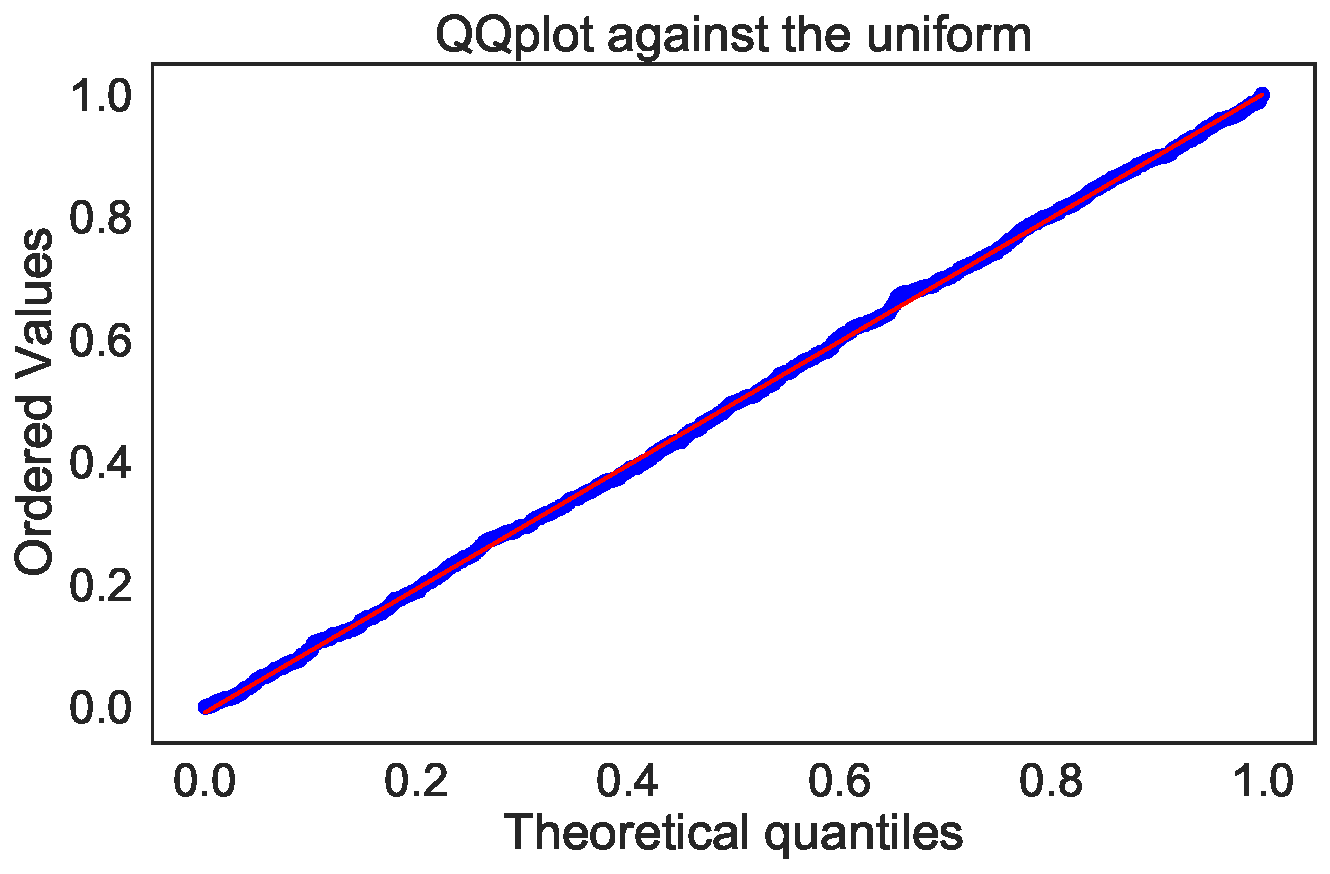
\includegraphics[width=\textwidth]{../results/QQplot.pdf}
         \caption{The QQplot against the uniform distribution in (0, 1) shows match. }\label{fig:lcgqq}
     \end{subfigure} \quad
     \begin{subfigure}{0.5\textwidth}
         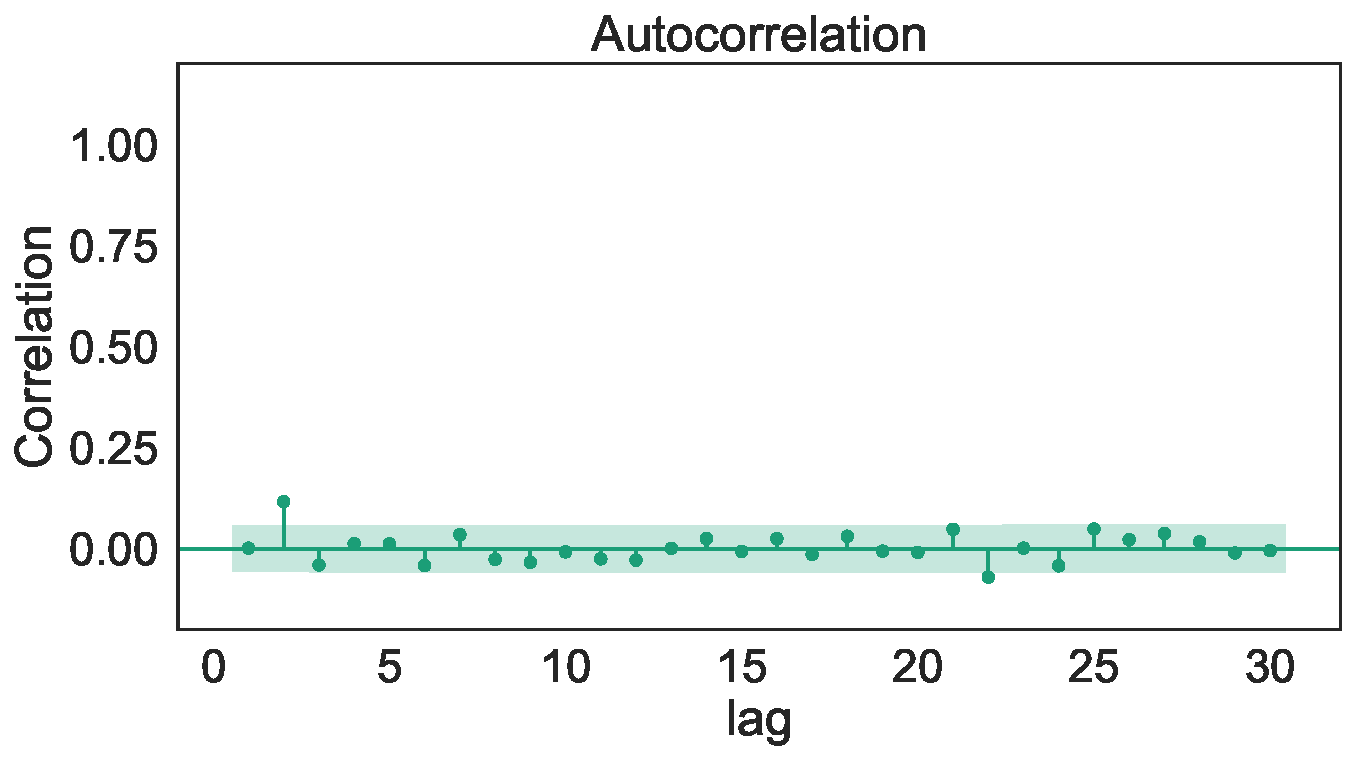
\includegraphics[width=\textwidth]{../results/autocorrelation.pdf}
         \caption{Autocorrelation plot does not highlight any correlation for all the lag considered. }\label{fig:lcgauto}
     \end{subfigure}
  \begin{subfigure}{0.9\textwidth}
         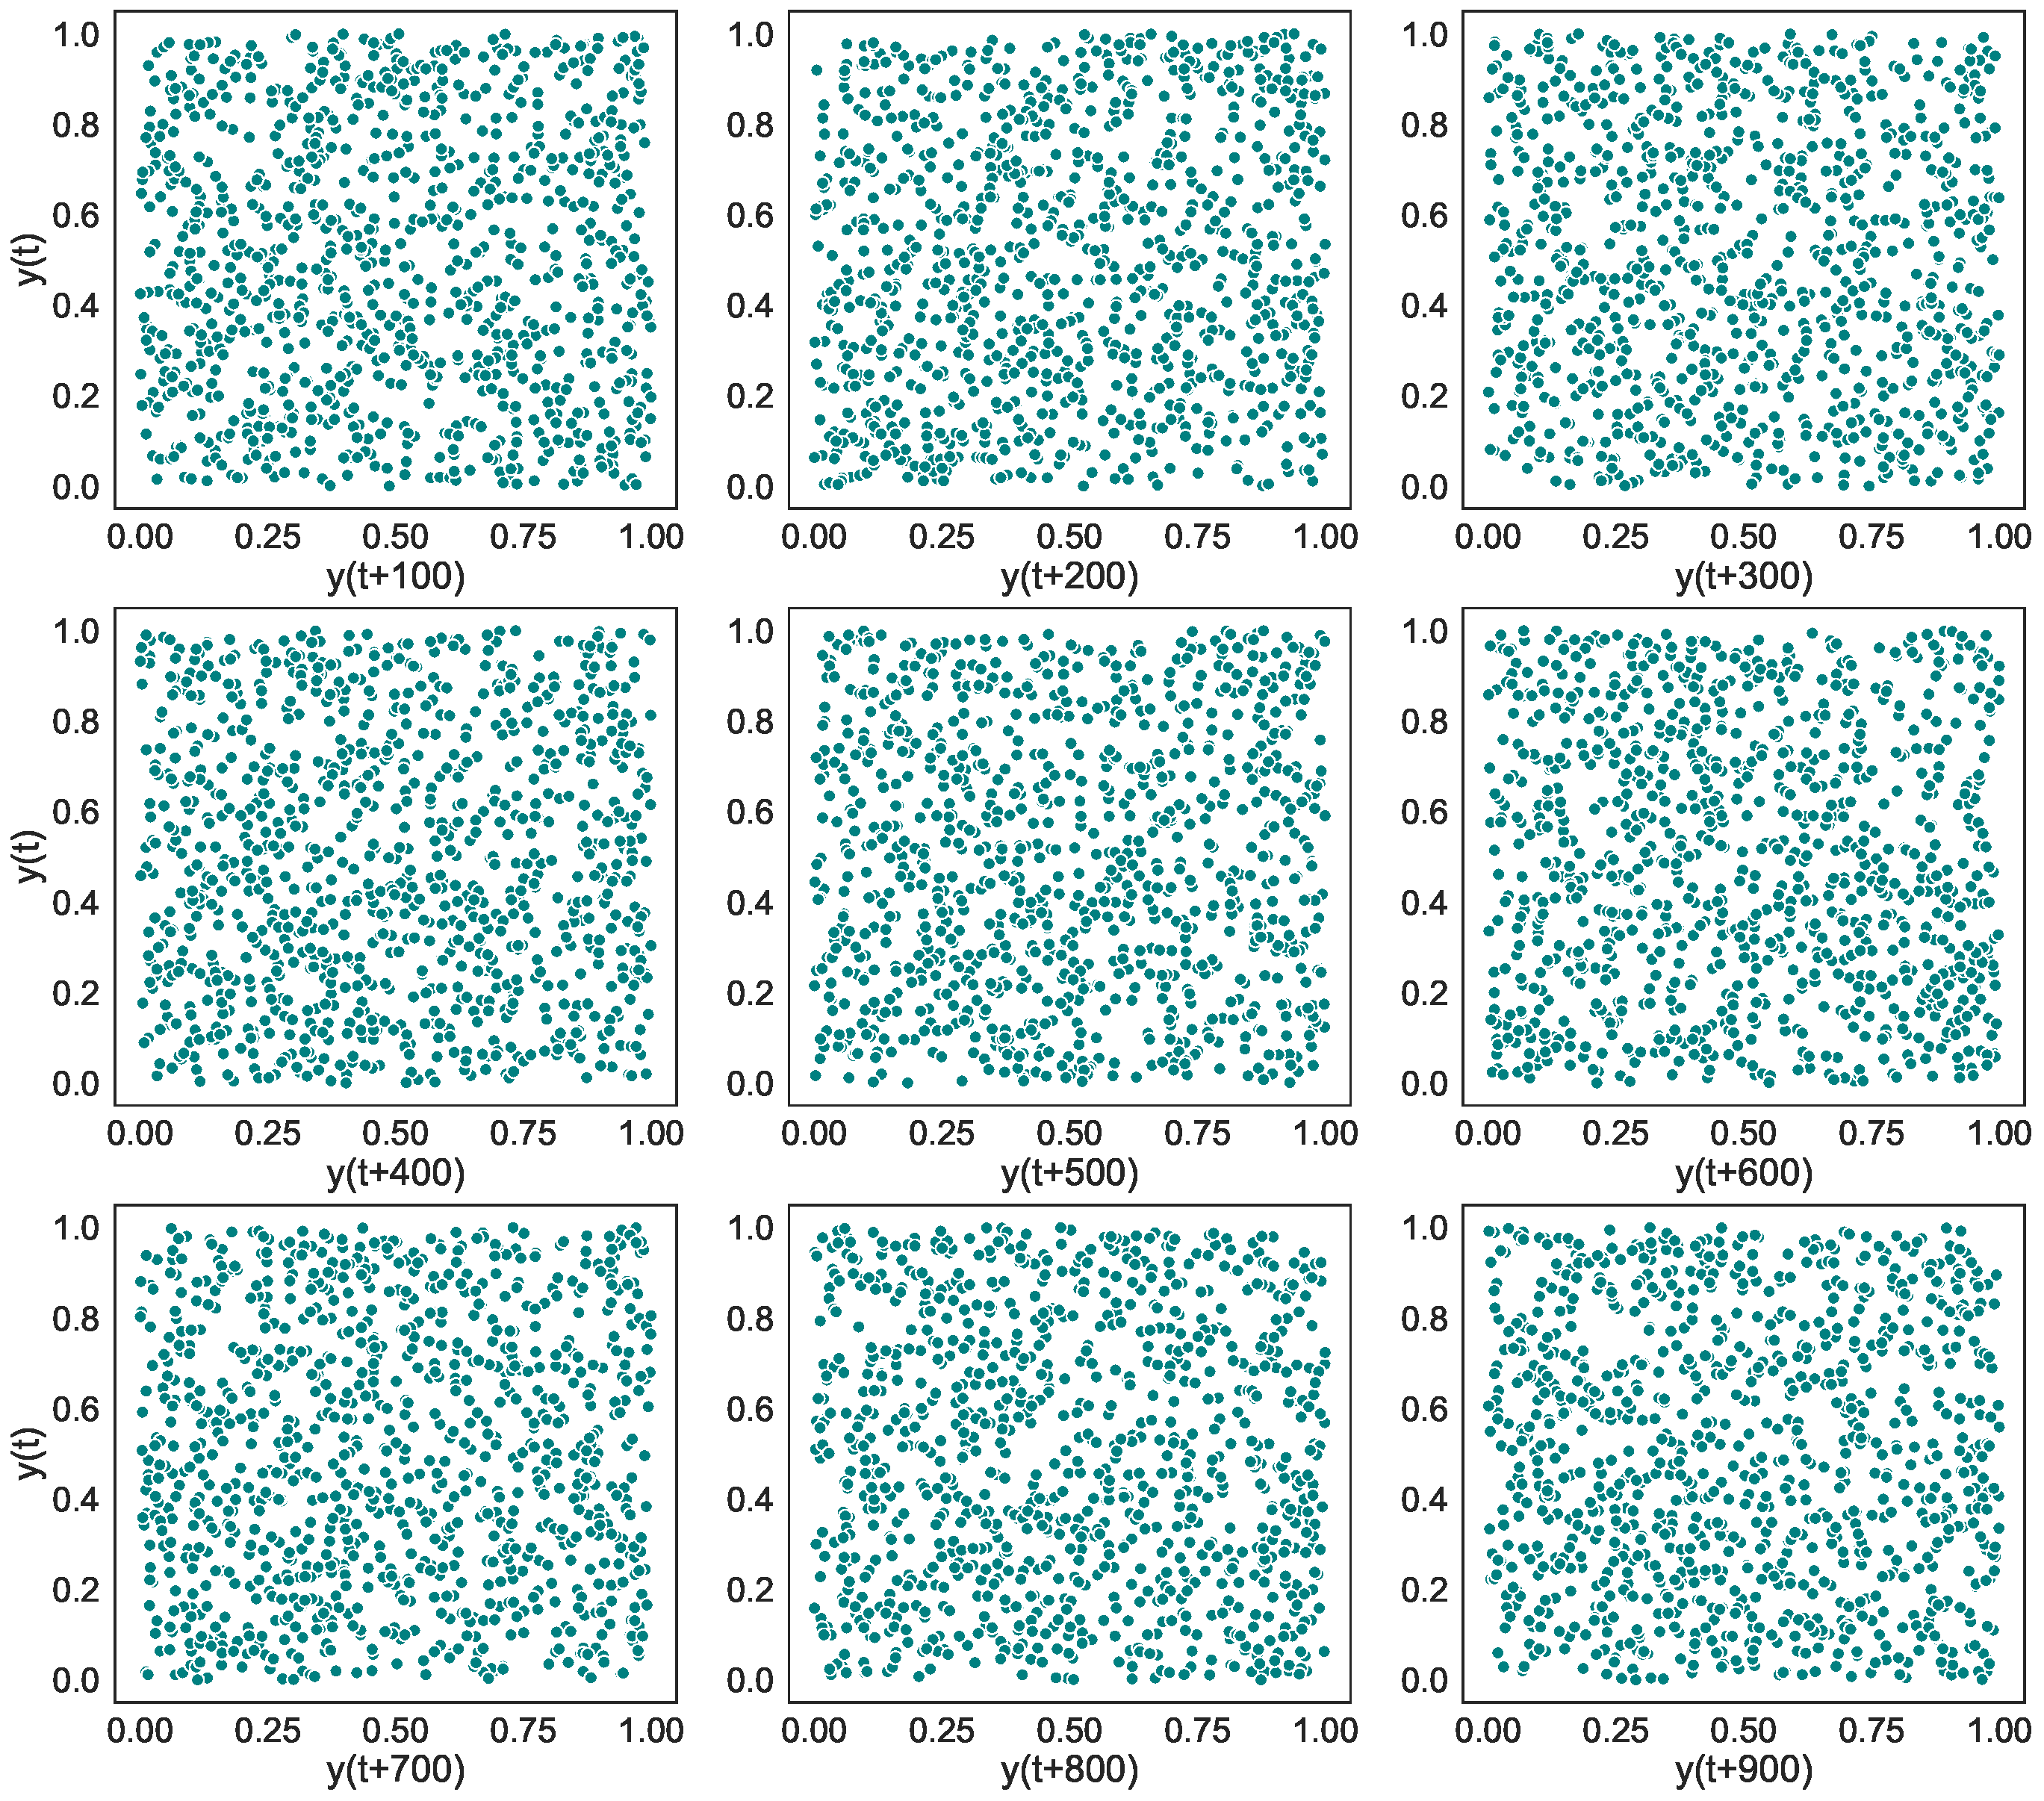
\includegraphics[width=\textwidth]{../results/lag_plots.pdf}
         \caption{Lag plots show that the sample is indeed independent.}\label{fig:lcglag}
     \end{subfigure}\caption{Sample of 1000 successive numbers uniformly distributed in $(0,1)$ with $a = 16807, \,\,m = 2^{31}- 1$. }\label{fig:lcg}
\end{figure}

\subsection{Seeding PRNGs}
An important point in generating random numbers is choosing a proper seed, in order to avoid the generation of periodic data and to have control over the simulation.
For instance, if we pick the last element of a first sample as seed for the next sample, we are sure that we won't generate a sequence with common elements, at least before reaching the periodicity.
To show the consequences of such choice we generate three samples of data: one with seed 1, one with seed 2, one with seed equal to the last element of the first sequence.
In Figure \ref{fig:seeds}, the left panel shows sequence with seed 1 vs seed 2, in the right panel $seed=0.6628$ is the last value of the sequence generated with seed 1.
It is clear that the first choice produces samples which are correlated, while in the second case we observe no correlation.

\begin{figure} \centering
         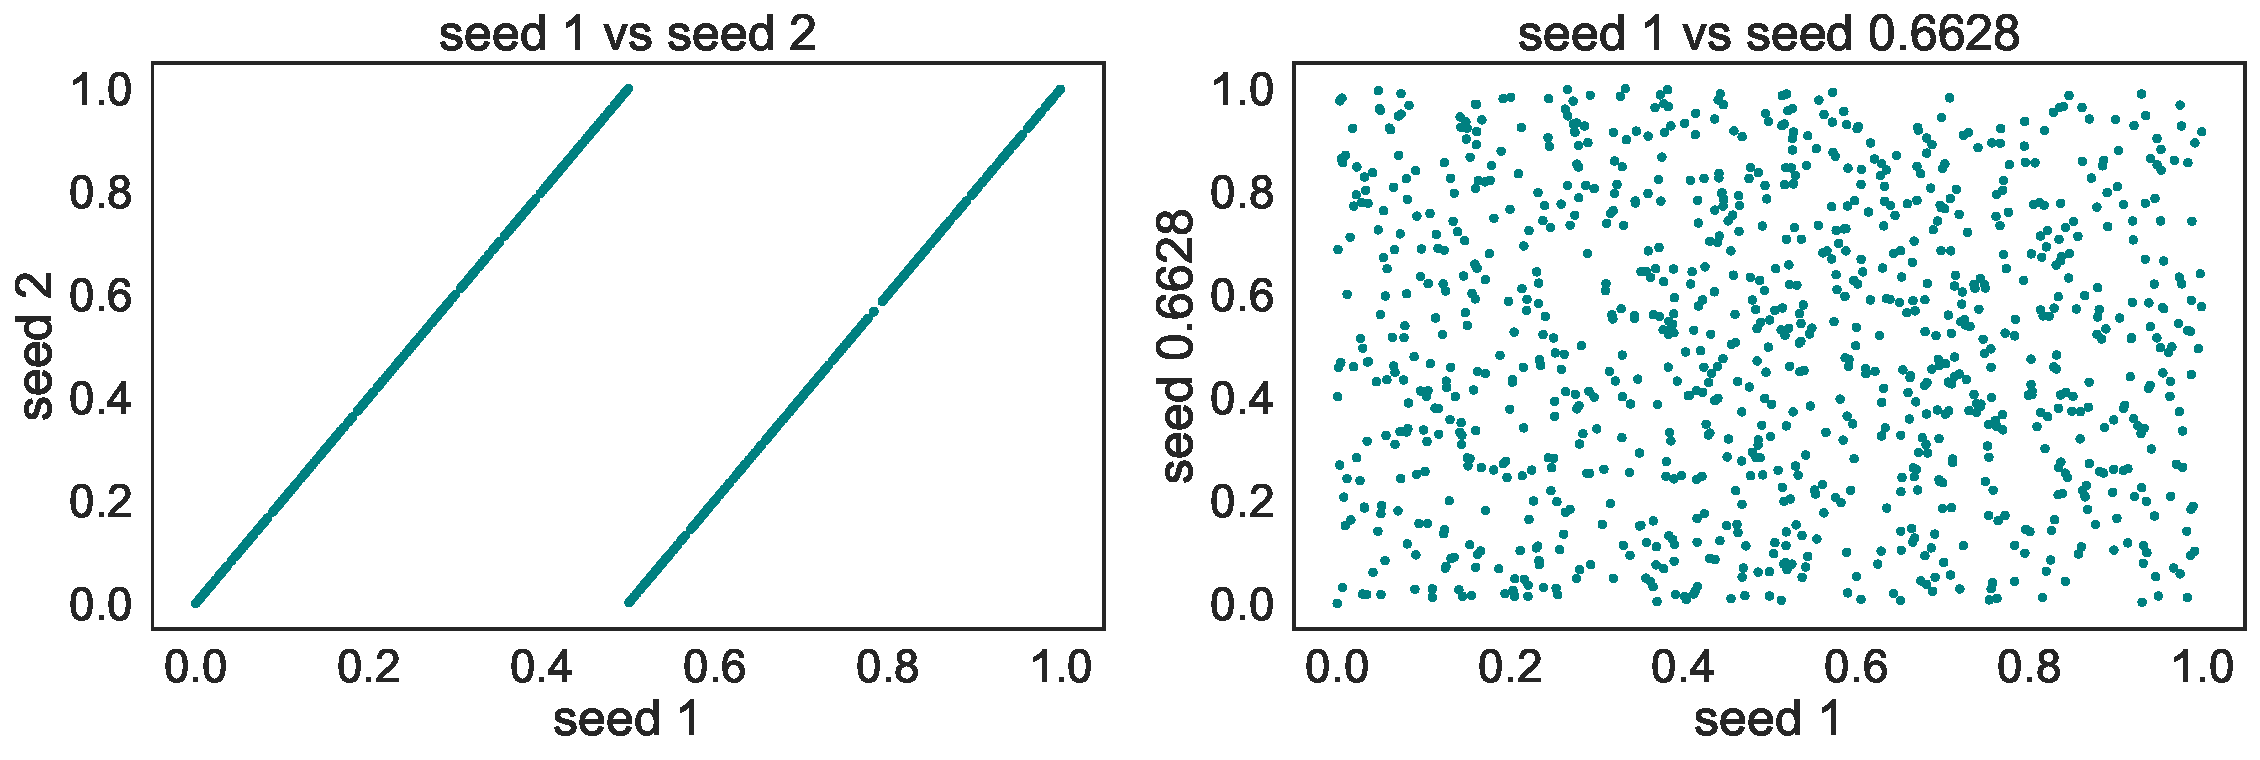
\includegraphics[width=\textwidth]{../results/seed_comparison.pdf}
\caption{Comparison of two samples generated with the same LCGs, but different seeds. The left panel shows results for seed 1 vs seed 2, the right panel shows seed vs a sequence generated with seed equal to  last value of first stream.}\label{fig:seeds}
\end{figure}

\subsection{Periodicity}
As we already pointed out, a problem related with LCGs is that these are characterized by a periodicity. The period can be at most m, but in general it depends on the combination of parameters, we refer to full period LCGs if the period $T=m$.
\par
Let us consider a first example of LCG with $a=18$ and $m=101$ and another one with  $a=2$ and $m=101$. 
We can manually deduce if these are full period or not by going through $m$ elements of the samples and check if the value has already been observed. We conclude that both of them are full period with period $m=101$.
To draw conclusion regarding the generation of pseudo random numbers with such tools, in Figure \ref{fig:params} we show all pairs $(U_i, U_{i+1})$ for both of them. It is possible to observe that the samples exhibit a regular behaviour with some clear patterns. The different arrangement of samples has to do with the value of $a$, since the parameter $m$ is shared among the two. Moreover, both of the LCGs are full period, thus plotting the first $m$ values we are displaying the entire space that can be generated from such generators. Indeed, the main issue that is possible to highlight from the plots is that the sequences are not independent. 

\begin{figure} \centering
         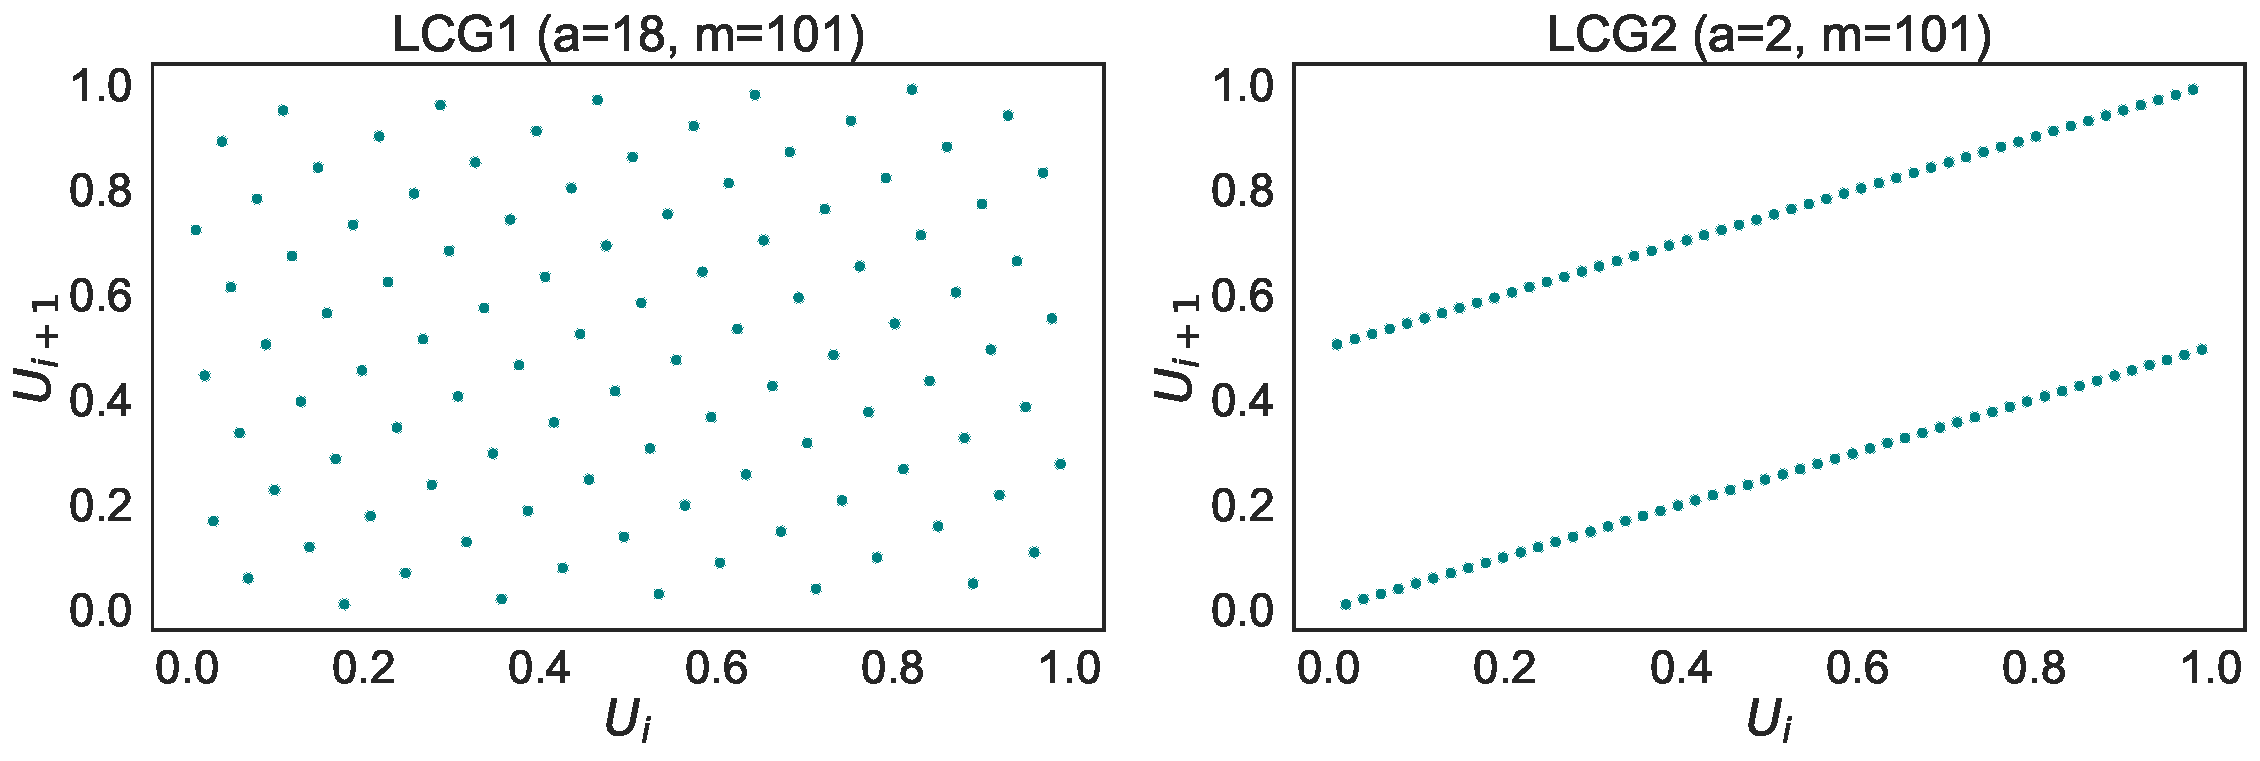
\includegraphics[width=\textwidth]{../results/lcg_params_study.pdf}
\caption{Scatterplot of $U_i$ vs $U_i+1$ for different LCGS. The left panel shows that the LCG with a=18 and m=101 exhibits a regular pattern. The right panel shows the correlation between consequent elements in a LCG with a=2 and m=101. }\label{fig:params}
\end{figure}
\par
Let us now consider another example, with  $a=65539$ and $m=2^{31}$. In Figure \ref{fig:unif_lcg} we show the pairs $(U_i, U_{i+1})$: from a two dimensional representation of data we would conclude that the sample consists of independent and uniformly distributed elements. Nevertheless, in Figure \ref{fig:3dlcg}, a 3-dimensional plot shows that, once we consider triples $(U_i, U_{i+1},U_{i+2})$, dependencies arise. 


\begin{figure} \centering
         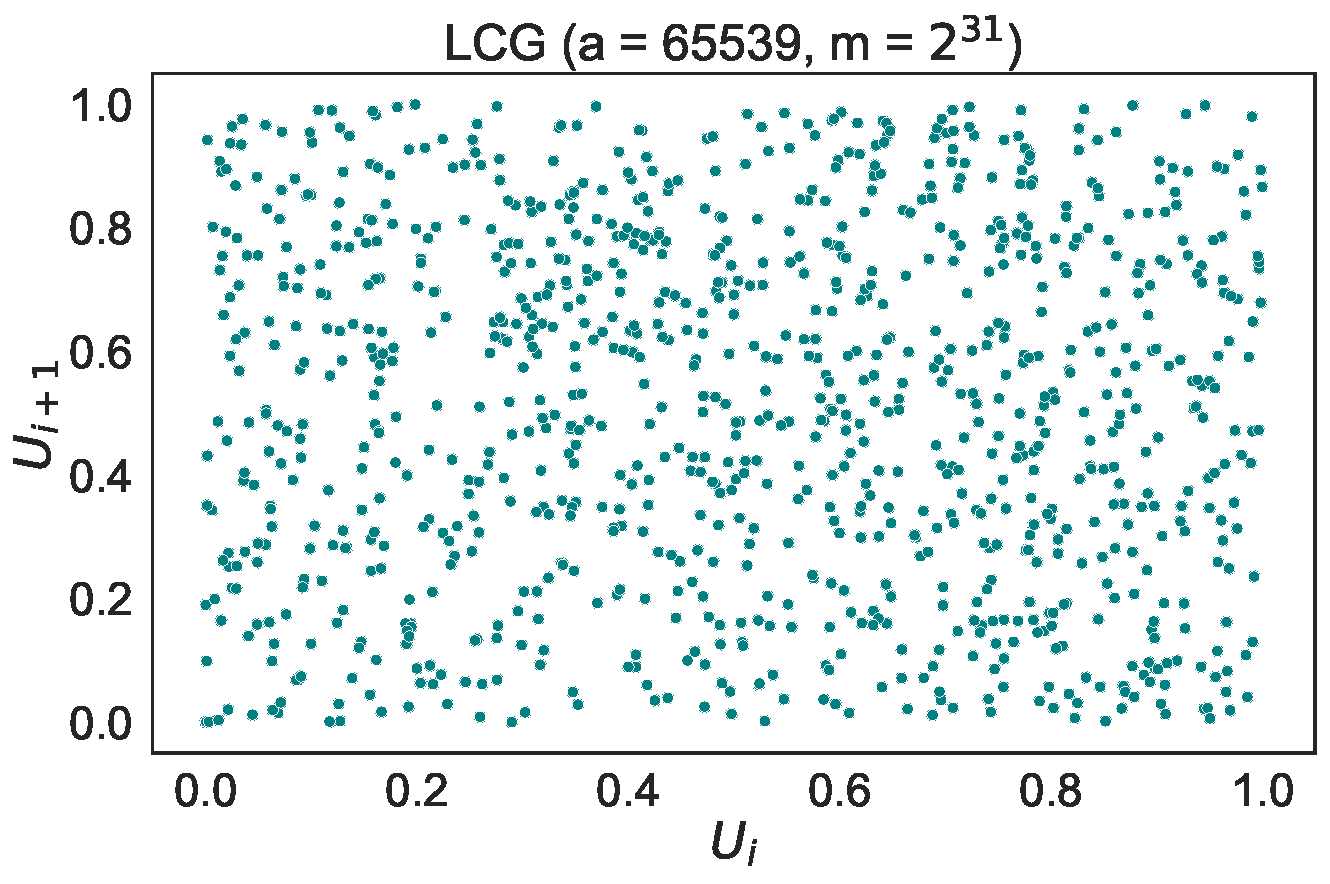
\includegraphics[width=0.6\textwidth]{../results/lcg_uniform.pdf}
\caption{Scatterplot of $U_i$ vs $U_i+1$ for a LCG with $a=65539$ and $m=2^{31}$, it shows that the sample is independent. }\label{fig:unif_lcg}
\end{figure}


\begin{figure} \centering
         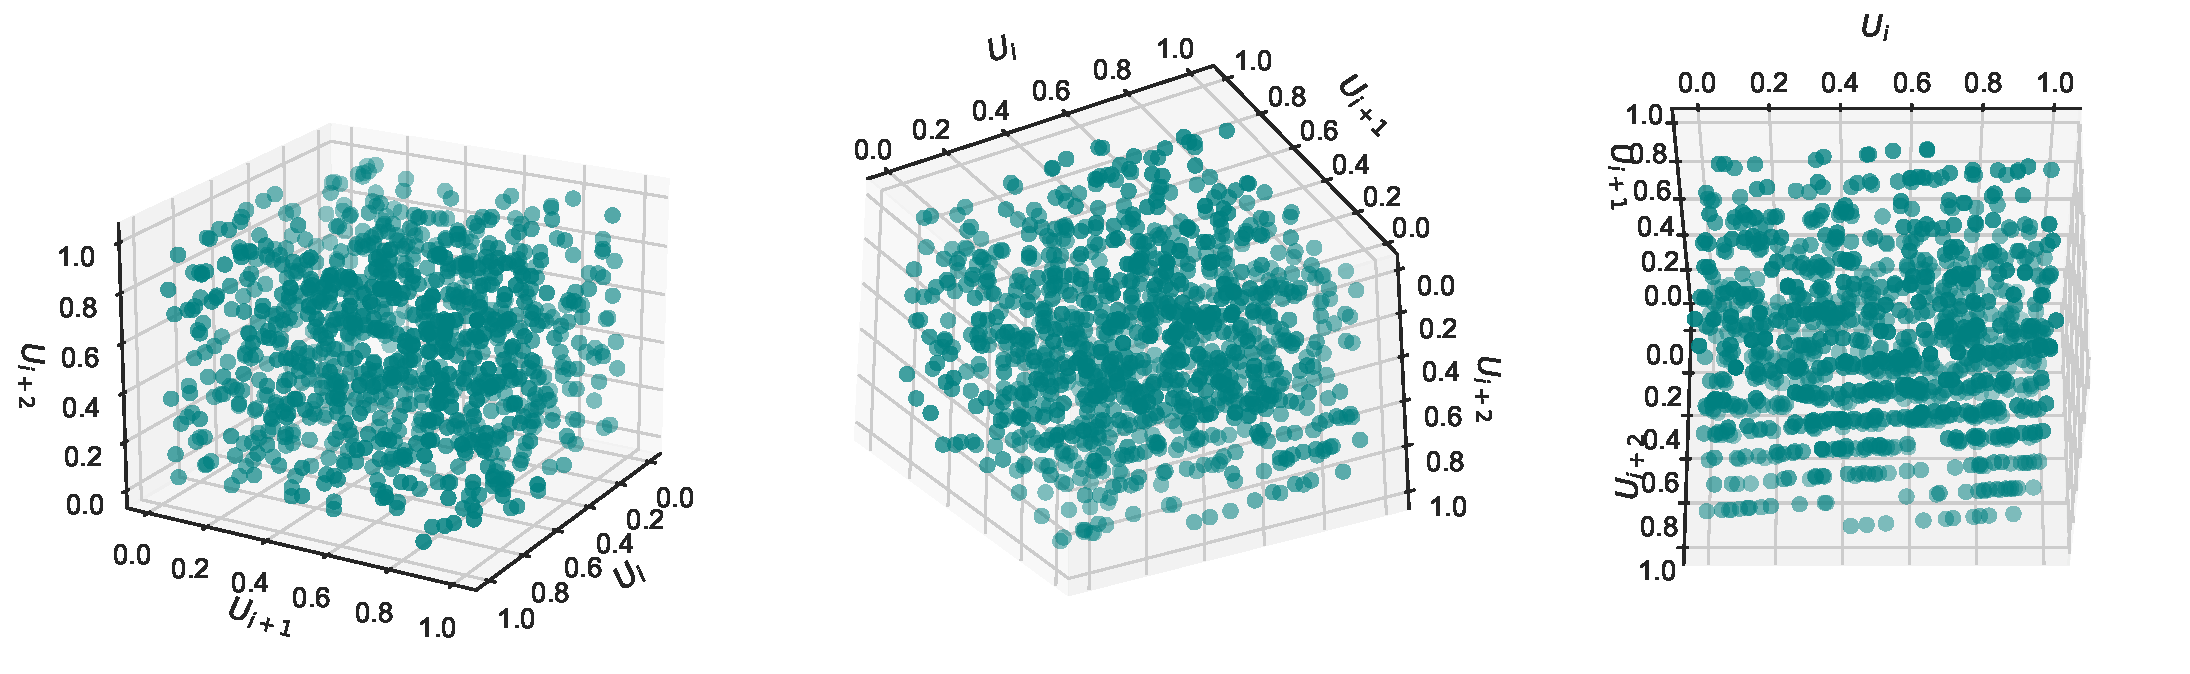
\includegraphics[width=\textwidth]{../results/lcg_3d.pdf}
\caption{3-dimensional representation of the sample generated with LCG with $a=65539$ and $m=2^{31}$, points are the triples $(U_i, U_{i+1},U_{i+2})$. It is possible to highlight that dependencies arise once one consider the third dimension. 
}\label{fig:3dlcg}
\end{figure}

\section{Generic distribution}
Since we already discussed methods and problems related to the generation of uniform random numbers, we now aim to exploit such observations to generate specific distributions. To this end, many approaches can be exploited, often based on the generation of a uniform value in $(0,1)$. here we propose a strategy based on rejection sampling.
\par
Let us consider a sample $Y$, which takes values in a finite interval $ [a,b] $. If its density is given by $f_Y = K \, f_Y^n$, where $K$ in un unknown normalization constant, thus $f_Y^n$ is the non normalized density, that we assume to be easy to compute. Let us also consider the case in which it is possible to find a bound $M: f_Y^n<M $. The algorithm \ref{alg:distr} shows the process in the 1-dimensional case, the generalization to the 2-dimensional is trivial.

\begin{algorithm}
\caption{Generation of RV with arbitrary distribution}\label{alg:distr}
\begin{algorithmic}
\State Take $U\sim(0,1)$,  $y\sim(0,M)$
\While {$U\geq f^n_Y$}
\State Take $U\sim(0,1)$,  $y\sim(0,M)$
\EndWhile
\State\Return $Y$
\end{algorithmic}
\end{algorithm}
In Figure \ref{fig:AR} we show two examples, in the left panel we provide the  histogram of 2000 samples of the distribution with $f_Y^n=\frac{sin^2x}{x^2}$, while in the right panel we show the 2-dimensional distribution with $f_{Y_1,Y_2}^n=|Y_2-Y_1|}$. Note that this method allows to generate a sequence without knowing the value of the normalization constant $M$.

\begin{figure} \centering
         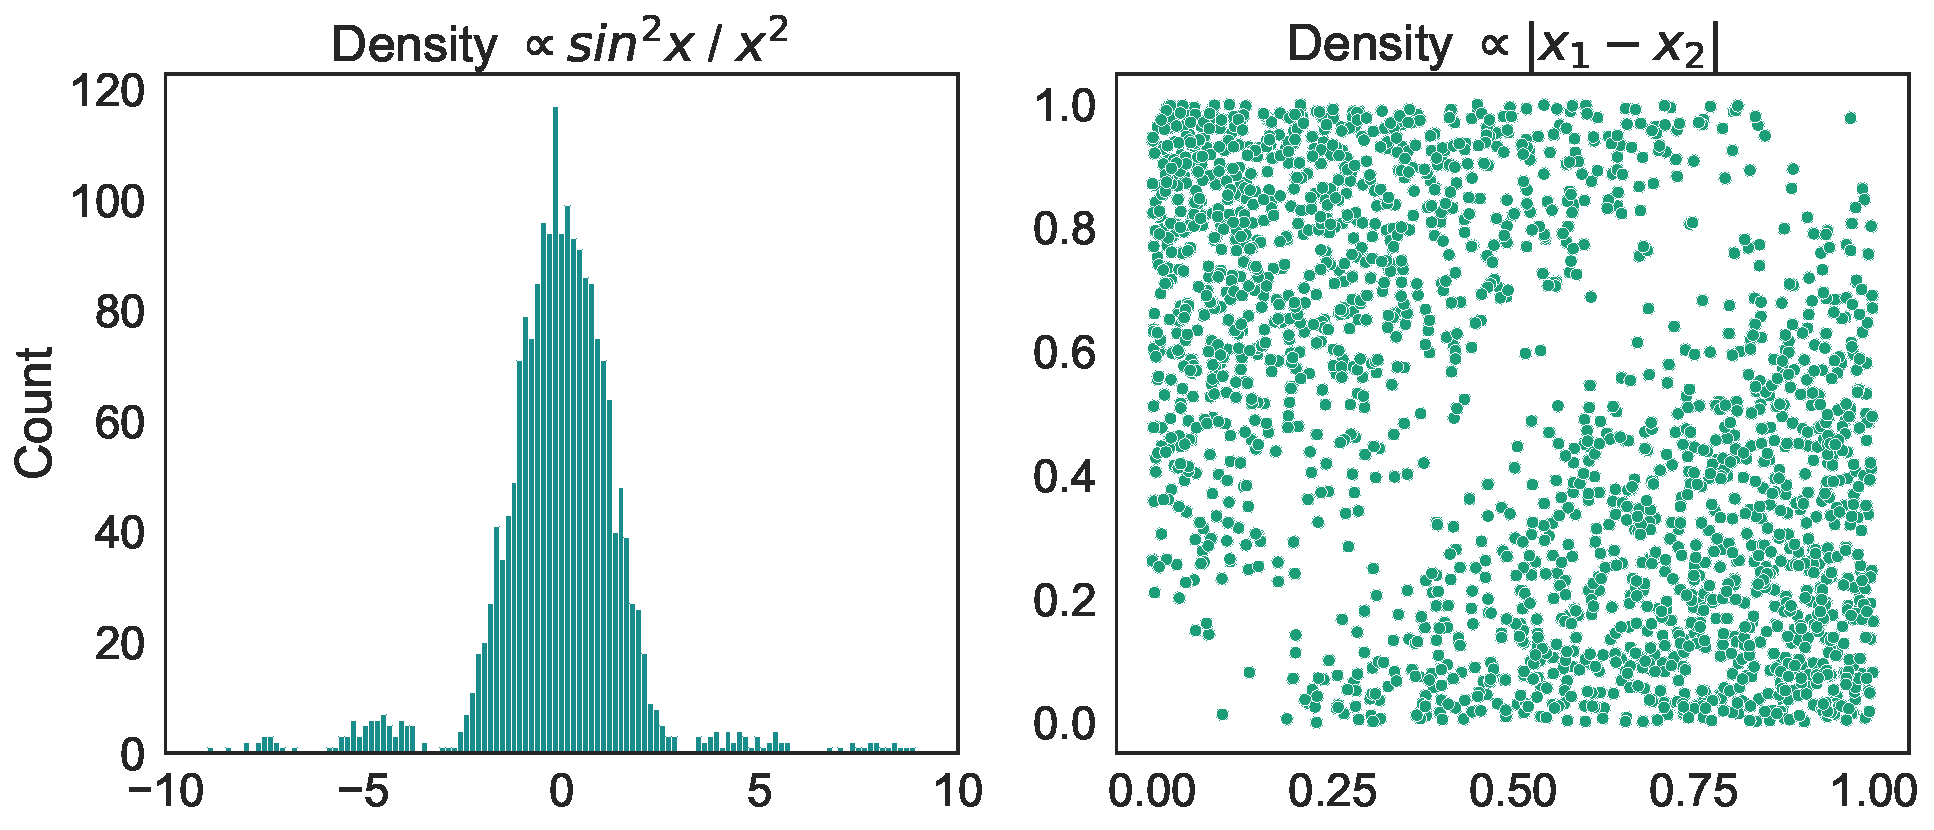
\includegraphics[width=\textwidth]{../results/AR.pdf}
\caption{Generated samples with arbitrary distribution. On the left panel we show 2000 samples of the distribution with $f_Y^n=\frac{sin^2x}{x^2}$, while in the right panel we show the 2-dimensional distribution with $f_{Y_1,Y_2}^n=|Y_2-Y_1|}$}\label{fig:AR}
\end{figure}

\section{Discrete random variables}
In this section we explore two specific discrete distributions: binomial and the poisson RVs.
\subsection{Binomial distribution}

A powerful approach to generate a specific distribution of RV is represented by CDF inverse method: the idea is that by generating samples uniformly in $(0,1)$ we are able to reconstruct a generic distribution  $F$ by exploiting the properties of the cumulative density function.
Formally, given $U\sim \mathcal U (0,1)$, then $\forall F$ continuous distribution function, the RV $X$ defined as $X=F^{-1}(U)$ is distributed as $F$. Such result can be extended to the discrete case and it can be applied efficiently to the generation of binomial samples because of the specific relationship that occurs between $B(n,k)$ and $B(n,k+1)$, the pseudo code is reported in Algorithm \ref{alg:bin}.


\begin{algorithm}
\caption{Generation of binomial RV}\label{alg:bin}
\begin{algorithmic}
\State Take $U$ uniformly in $(0,1)$
\State $c=\frac{p}{1-p}$
\State $i=0$
\State $pr=(1-p)^n$
\State$F=pr$
\While {U\geq F}

 \State$pr = pr\,\,{c(n-i)/(i+1)}$
\State $F=F+pr$
\State $i=i+1$
\EndWhile

\State$ X=i$
\State\Return $X$
\end{algorithmic}
\end{algorithm}

Another method to generate binomial RV with parameters $n,p$ is to pick a value $ u \sim \mathcal U(0,1)$ $n$ times, and count the number $k$ of successes of the event $u<p$. $k$ corresponds indeed to the definition of binomial RV.\par
Finally, we could also consider a binomial process as a sequence of extractions of geometric RV. Indeed, a geometric RV with parameter $p$ represents the number of trials one has to go through before observing a successful event. We can then count the number $k$ of geometric RV that it is necessary to generate in order to collect $n$ trials. Still,  $k$ is a binomial RV.



\begin{figure} \centering
         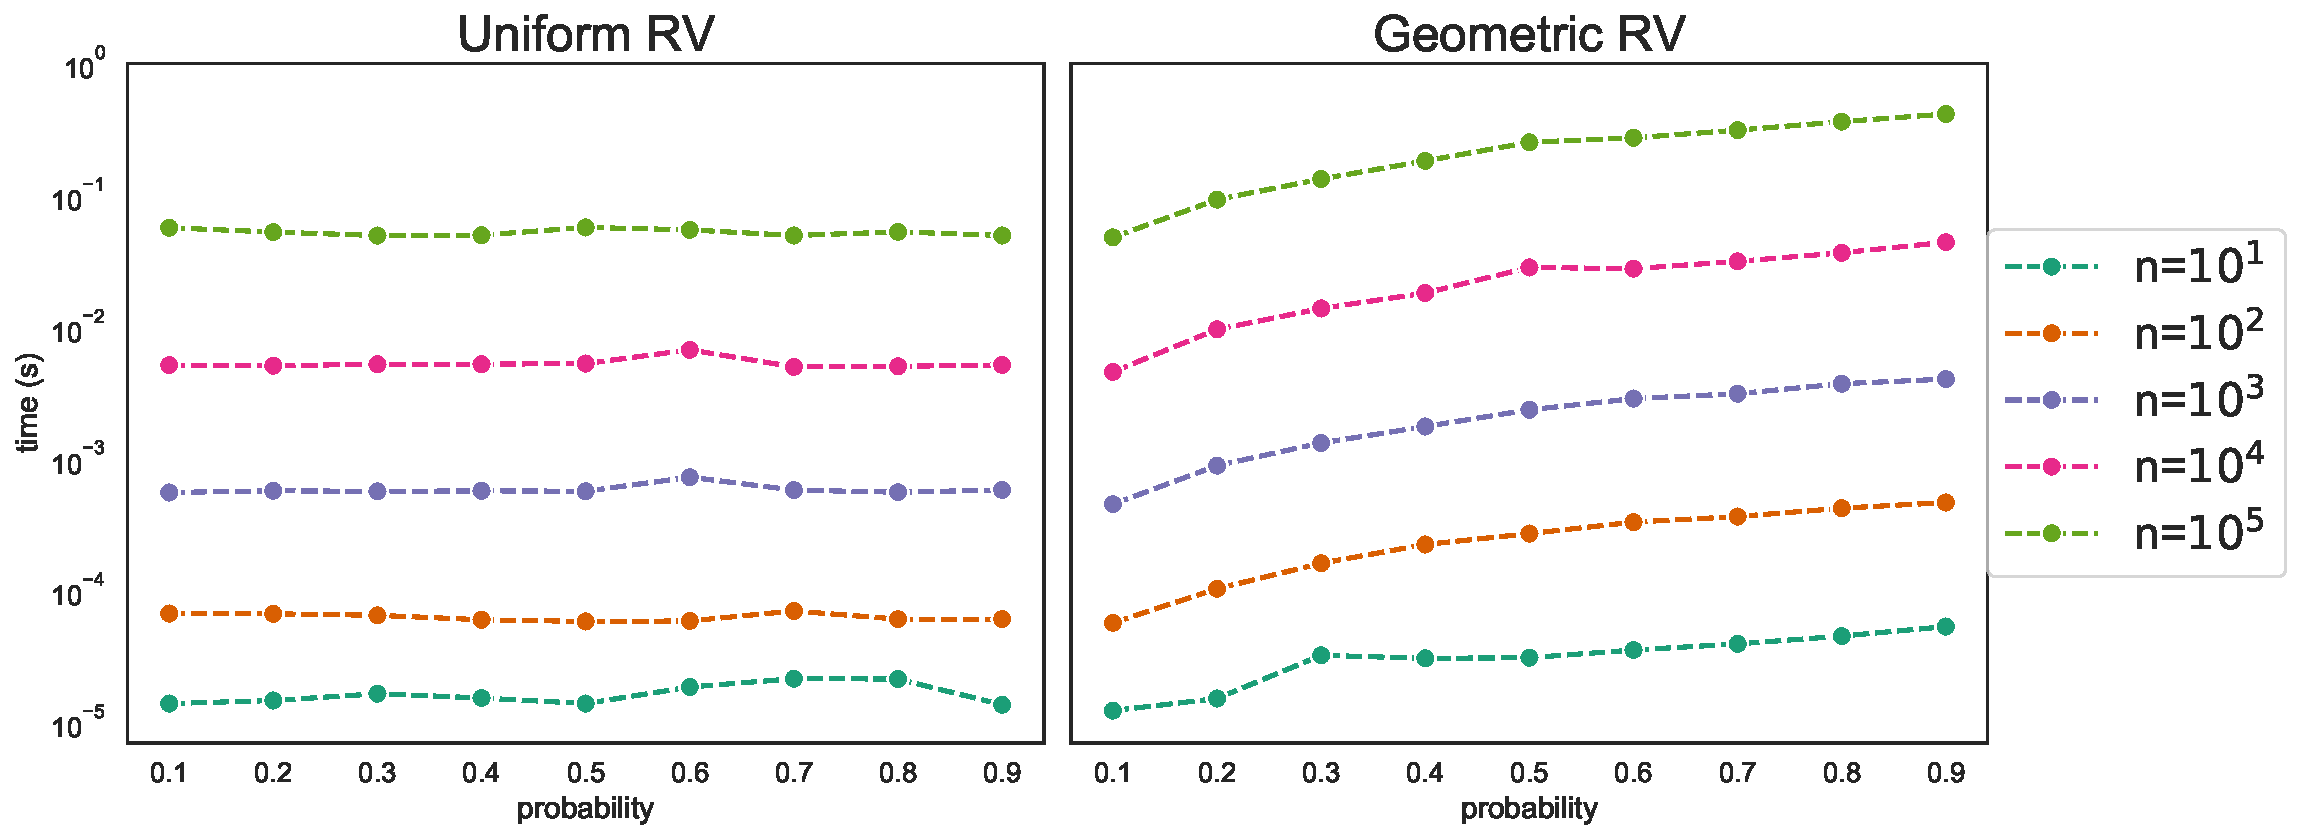
\includegraphics[width=\textwidth]{../results/binomial_time_unif_cdf.pdf}
\caption{Time necessary to generate a binomial RV with the method that exploits uniform distribution (left panel) and geometric distribution (right panel). We provide results in logarithmic scale, for different values of n, as a function of p.}\label{fig:bin}
\end{figure}

\begin{figure} \centering
         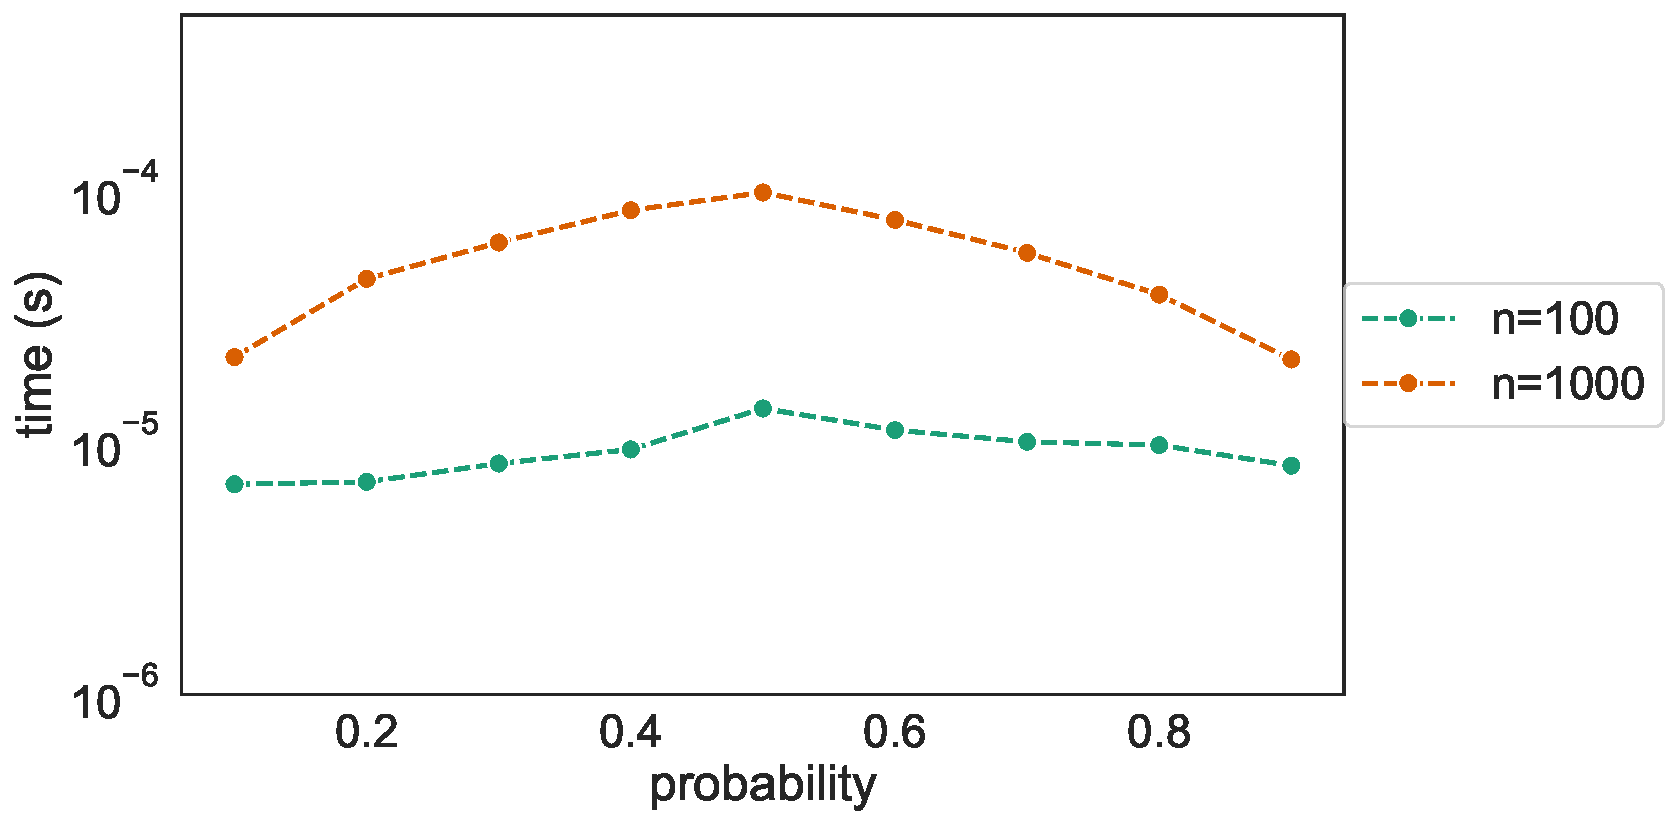
\includegraphics[width=0.7\textwidth]{../results/binomial_time_cdf.pdf}
\caption{Time necessary to generate a binomial RV with CDF method.}\label{fig:bin_cdf}
\end{figure}

To test the performances or our generator, we generate $100$ RV for different values of $n$ and $p$, compute the time for each generation and take the average over $N$.
In Figure \ref{fig:bin} we show the result, in logarithmic scale, for different values of $n$ and $p$. It is possible to conclude that the time needed to sample RV with the method based on uniform RV increases with $n$, while it is constant with $p$. We would expect such result since time is connected only to the number of uniform RV that must be extracted to generate a single binomial variable,  $n$, but not on the probability, which is used only to check if the event occurs.
On the other hand, using geometric RV time increases both with $n$ and $p$. This behaviour can be explained if we consider that the bigger $n$, the more geometric RV we have to generate, moreover if $p $ increases, the sequence of trials becomes shorter thus we need to generate more variables as well.
Finally, in Figure \ref{fig:bin_cdf} we provide, for two values of $n$, the time necessary to generate our sequence of data with CDF method. In this case we extended Algorithm \ref{alg:bin}, by exploiting a backward approach to address probabilities greater than 0.5. It turns out, as we expect, that the worst case scenario corresponds to $p=0.5$, since it is the furthest point both starting from 
zero and $n$ successes. Moreover, we observe that time increases with $n$ as expected.


\subsection{Poisson distribution}
The CDF method is generic, thus it can also be exploited in order to generate poisson RV, in Algorithm \ref{alg:pois} we provide the adaption of CDF algorithm to the generation of poisson RV. 

\begin{algorithm}
\caption{Generation of Poisson RV}\label{alg:pois}
\begin{algorithmic}
\State Take $U$ uniformly in $(0,1)$
\State $i=0$
\State $p=e^{-\lambda}$
\State$F=p$
\While {U$\geq$ F}
 \State$p = p\lambda(i+1)$
\State $F=F+p$
\State $i=i+1$
\EndWhile

\State$ X=i$
\State\Return $X$
\end{algorithmic}
\end{algorithm}
Nevertheless, it is possible to design other methods to generate poisson RVs, which are based on the generation of exponential RVs, since the distribution of interarrival times in a poisson process is exponential. A poisson RV represents indeed the number of occurrences of an event, i.e. arrivals, in a given interval of time. As a consequence, for a unitary interval, a poisson RV is given by:
\begin{equation}
N = \max_n\{n: \sum_i^n x_i \leq 1\}, 
\end{equation}
where $x_i$ has exponential distribution with parameter $\lambda$, thus it can be generated as follows:
\begin{equation}
x_i = \frac{\log u}{\lambda}, \quad u\sim \matchal U(0,1).
\end{equation}
Finally, the previous method can be optimized by rewriting the previous formula as:
\begin{equation}
N = \max_n\{n: \prod_i^n u_i \leq e^{-\lambda}\}, \quad u_i\sim \matchal U(0,1).
\end{equation}
To test the performances, as we did with the binomial distribution, we generate $100$ RV for different values of $\lamda$, compute the time for each generation and take the average over $N$. In Figure \ref{fig:poisson_time} we show results of the simulation: it is possible to observe that time increases with $\lambda$ for all the considered methods. In particular, the most efficient method is the CDF based, while exponential RV generation requires more time.


\begin{figure} \centering
         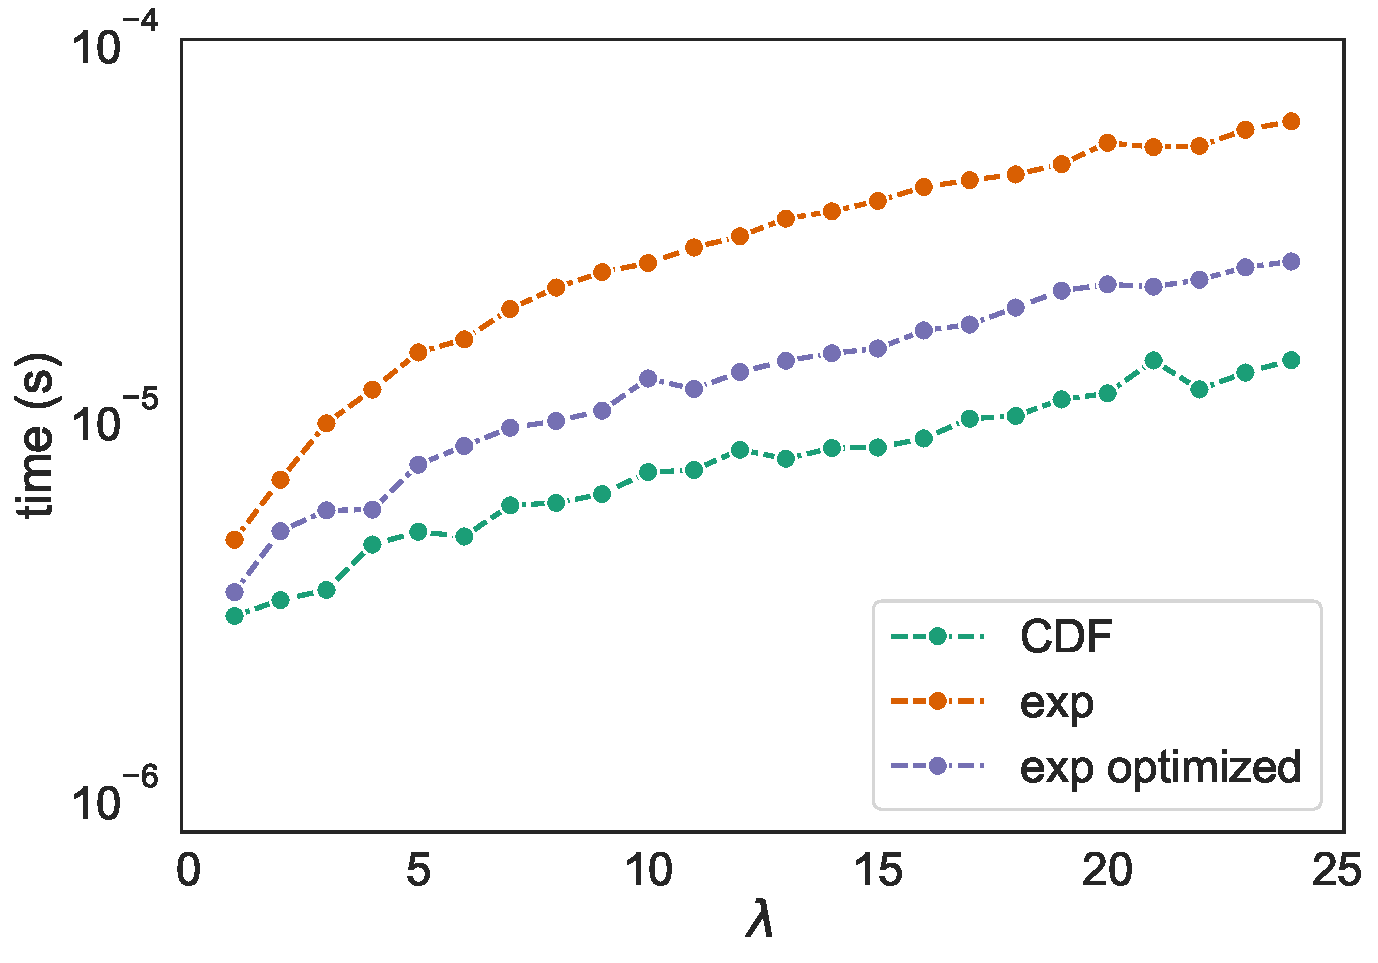
\includegraphics[width=0.7\textwidth]{../results/poisson_time.pdf}
\caption{Time necessary to generate a poisson RV with the methos discussed. We provide results in logarithmic scale, as a function of $\lambda$.}\label{fig:poisson_time}
\end{figure}


\end{document}

